\chapter{Definitions}

Since the main concern of this thesis is coloring of the graphs mentioned in the preface, it is useful to define all the necessary concepts we will be working with.

\section{Basic definitions and assumptions}

Here we state mathematical definitions, that should not be surprising in any way. Also, we state some assumption we will make, which will then hold for the rest of this thesis.

\begin{definition}
    An \textit{undirected graph} $G$ is an ordered pair $G=(V,E)$ where $V$ is a set of vertices of the graph and $E \subseteq \binom{V}{2}$ is the set of its edges. 
\end{definition}

\begin{assumption}
    For any graph $G=(V,E)$ we will assume $V \cap E = \emptyset$. 
\end{assumption}

\begin{definition}
    A \textit{partial function} is a function $f:X \rightarrow Y$ s.t. $\forall x \in X$ we have $f(x) \in Y$ or $f(x)$ is undefined.
\end{definition}

\begin{highlight}
Since we are interested in Platonic and Archimedean solids, whose graphs are all planar, it is useful to define the notion of a \textit{plane graph}. This notion will correspond to a drawing of a particular graph onto a plane with one special property: the edges as they are drawn do not cross.

\begin{definition}
    Let $G=(V,E)$ be a graph. We call function $\varphi : V \cup E \rightarrow \mathbb{R}^2$ a \textit{drawing} of $G$ if it satisfies the following properties:
    \begin{enumerate}
    
        \item $\forall e=\{u,v\} \in E : \varphi(e)$ is a continuous line $\gamma$ whose endpoints are $\varphi(u)$ and $\varphi(v)$ such that $\gamma$ does not cross itself.
        
        \item (different vertices not drawn on same point) \\ $\forall u,v \in V : u \neq v \implies \varphi(u) \neq \varphi(v)$
        
        \item (edges not drawn onto non-endpoint vertices) \\ $\forall v \in V, \forall e \in E: v \notin e \implies \varphi(v) \notin \varphi(e)$
        
        \item (different edges can share only their common endpoints) \\ $\forall e \neq f \in E : x \in \varphi(e) \cap \varphi(f) \implies x = \varphi(v)$ and $v = e \cap f$
    \end{enumerate}
\end{definition}

A drawing of a graph might split the plane $\mathbb{R}^2$ into multiple separate segments. We will call these segments \textit{regions} of a drawing of graph $G$.

\begin{definition}
    A graph $G$ is \textit{planar} if there exists a drawing of $G$ into a plane.
\end{definition}

\begin{definition}
    A \textit{plane graph} $G' = (V,E,F)$ is a drawing of a planar graph $G=(V,E)$ into plane $\mathbb{R}^2$ where $F$ is the set of all regions of this drawing. 
\end{definition}

\end{highlight}

\section{The general concept of coloring}

As we will be working with many different colorings, to avoid repetition, we will define the notion of an abstract coloring which all the particular colorings will share.

\todo[inline]{JF: nevím, jestli někdy nebudete chtít barvit i stěny třeba v tzv. perfect coloring.
Pěkný přehled o barveních je zde: \url{https://fs.unm.edu/IJMC/Graph_Coloring,Types_and_Applications_A_Survey.pdf} 
}

\begin{definition}
    For $k \in \mathbb{N}$ and a graph $G=(V,E)$ \textit{coloring} of $G$ is a partial function $c: V \cup E \rightarrow \{1,\ldots,k\}$ with a coloring rule $R$ that restricts, which elements of the graph cannot share the same color.
\end{definition}

\todo[inline]{JF: Zvažte, jestli obecné obarvení neuvést třeba nějak jako:

The concept of coloring is in mathematical sense equivalent to the concept of mapping, when the domain --- the set of colors --- is usually a finite set without any further structure. So the only relevant characteristic is, whether two elements are mapped on the same target, or to phrase less colloquially: colored by the same color.

Hence we may without loss of generality assume that the domain is a set of positive integers, however sometimes we use usual colors like \emph{red}, \emph{blue}, etc, to visualize some particular colorings in more accessible way.
}

In other words, coloring is an assignment of numbers to vertices, edges or both s.t. based on the coloring rule, certain vertices or edges cannot share the same color. The coloring rule is usually independent on the choice of graph.

\begin{definition}
    Let the set of all colorings sharing the same coloring rule $R$ be called a \textit{family of colorings}.
\end{definition}

%\begin{highlight}
\begin{definition}
    Let $G=(V,E)$, let $F$ be a family of colorings, let $k \in \mathbb{N}$. \\ A function $c \in F$ such that $c: V \cup E \rightarrow \{1,\ldots,k\}$ is called a \textit{k-coloring} of $G$.
\end{definition}

Note that a $k$-coloring does not necessarily have to use all of the $k$ available colors. Mathematically speaking, a $k$-coloring is not necesserily a surjective function.

\begin{definition}
    For a graph $G=(V,E)$, family of colorings $F$ and a natural number $k$, if there exists a k-coloring of $G$ then we say that $G$ is \textit{k-colorable}.
\end{definition}

    A typical question we ask ourselves when considering colorings of graph is: What is the least amount of colors we can use to color the graph, without breaking the coloring rule? This leads to a definition of so called \textit{chromatic number}. 
%\end{highlight}

\begin{definition}
    For a graph $G$ and a family of colorings $F$, let \textit{chromatic number} $\chi ^F (G)$ be the minimum $k \in \mathbb{N}$ s.t. $G$ is k-colorable.
\end{definition}

%\todo[inline]{JH: Přidána poslední věta}
Once we know a graph is k-colorable, there is another interesting property of the graph we can examine. We can ask about how many different colorings with k colors there exists for the given graph. A closely related concept to this question is the \textit{chromatic polynomial}. But first, we need to define what it means for to colorings to be different.

\begin{definition}
    Given a graph $G=(V,E)$, family of colorings $F$ and k-colorings $c_1,c_2 \in F$: $c_1$ and $c_2$ are different if there exists $x \in V \cup E$ s.t. $c_1(x) \neq c_2(x)$.
\end{definition}

The definition above states, that if two colorings assign some element a different color, then the colorings are considered different. Note that this does not take into account any symmetries of the graph.

\begin{definition}
    For graph $G$ and a family of colorings $F$, the \textit{chromatic polynomial} denoted by $P^{F}_G(x)$ is a function s.t. $\forall k \in \mathbb{N} : P^{F}_G(k) = n$, where $n$ is the number of different k-colorings of $G$.
\end{definition}

For example, given the graph of tetrahedron $K_4$, the chromatic polynomial $P^{F_V}_G(x) = x \cdot (x-1) \cdot (x-2) \cdot (x-3)$. This can be seen if we label the vertices $v_1,v_2,v_3,v_4$ and imagine coloring them sequentially in the order of their labels. We have exactly $x$ colors left to use for the first vertex. With each other vertex, we have one less color available to use. 

\section{Particular types of colorings}

\subsection{Vertex coloring}

\begin{definition}
    A \textit{vertex coloring} of a graph $G=(V,E)$ is a coloring $c : V \rightarrow \mathbb{N}$ belonging to family of colorings with the following coloring rule:
    \begin{equation}\label{eqn:vtx_rule}
        \forall u,v \in V, \quad \text{if } \{u,v\} \in E, \text{ then } c(u) \neq c(v). 
        \tag{$R_V$}
    \end{equation}
    We will denote this family of colorings by $F_V$.
\end{definition}

In other words, vertex coloring is an assignment of colors to each vertex s.t. no two vertices connected by an edge share the same color.

\begin{figure}[H]
    \centering
    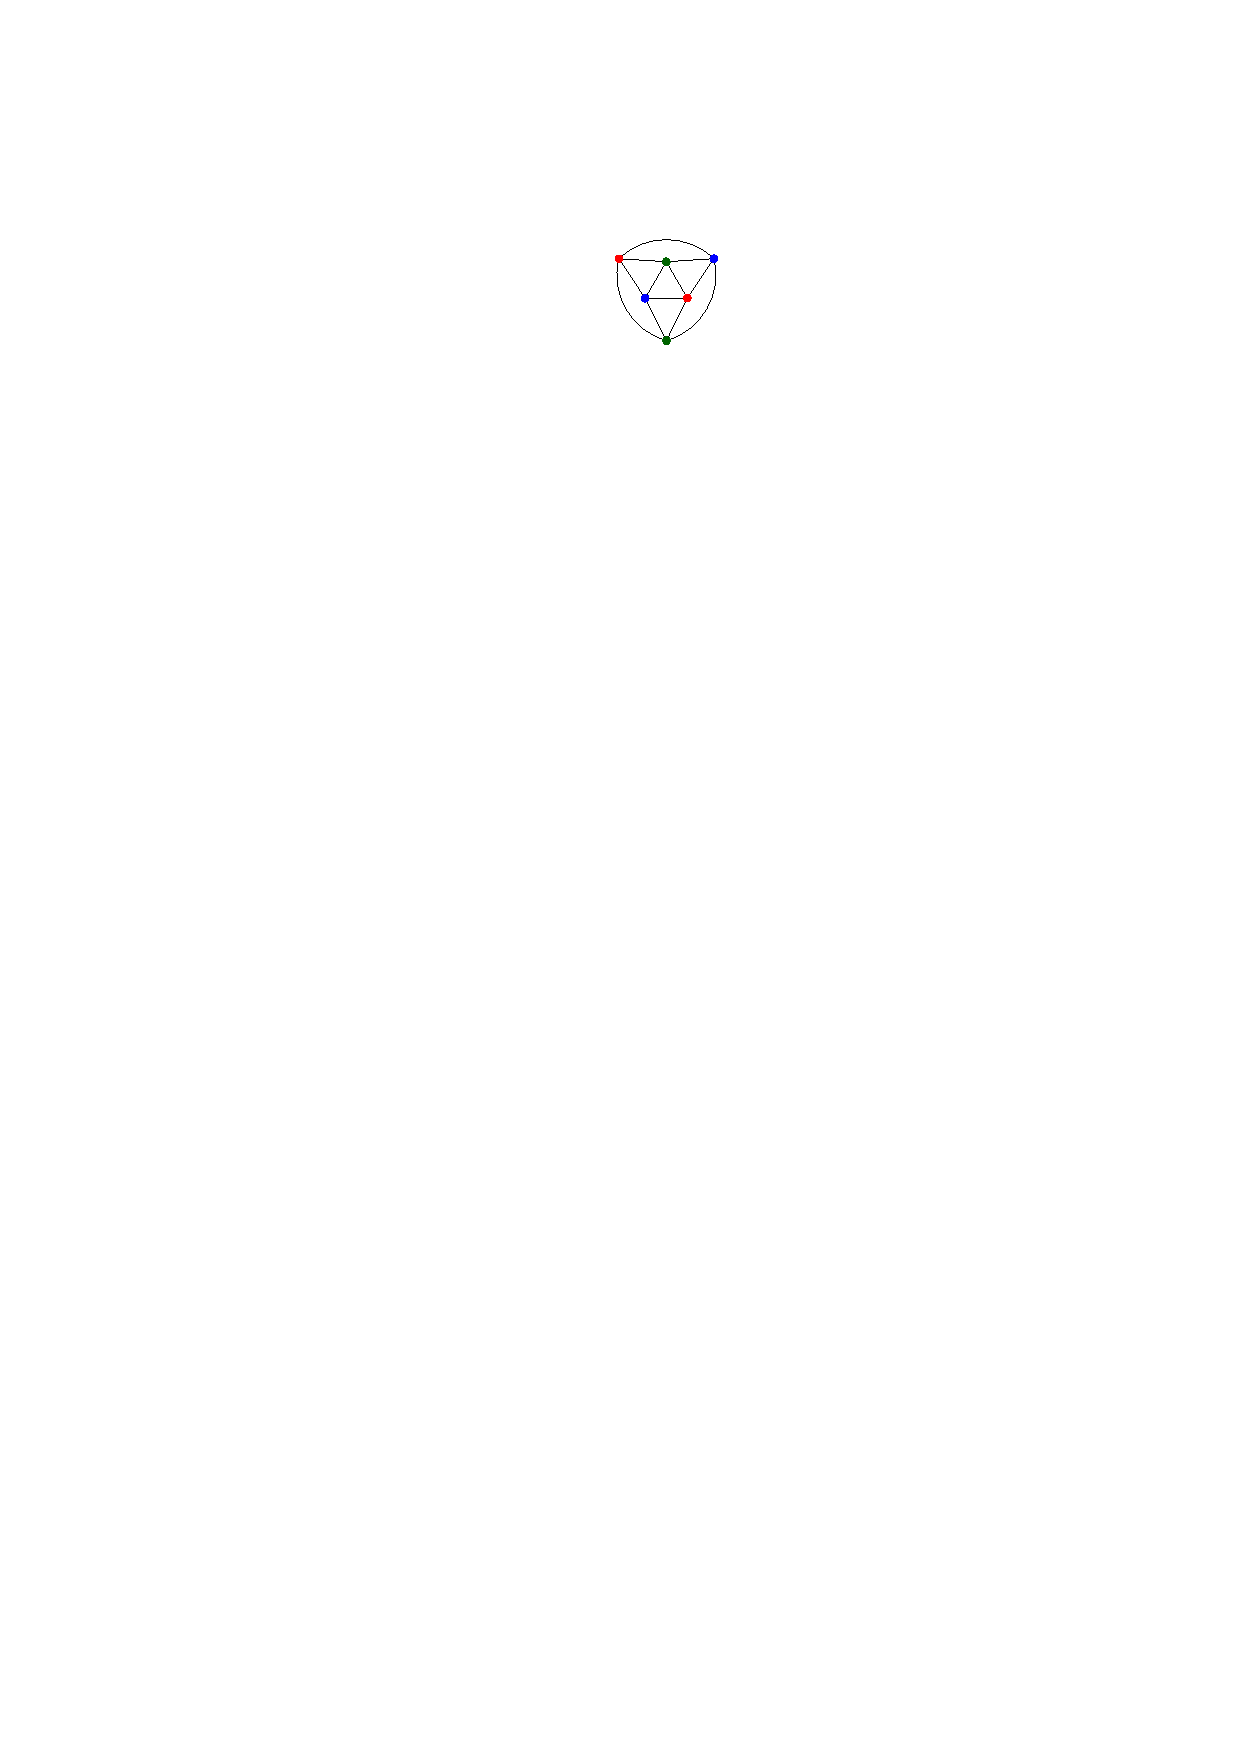
\includegraphics[width=0.2\textwidth]{../Resources/Figs/octahedral_vtx_colr.pdf}
    \caption{Vertex coloring of octahedral graph}
    \label{fig:octahedral_vtx_coloring}
\end{figure}

The graph in figure~\ref{fig:octahedral_vtx_coloring} has vertex chromatic number 3.

\subsection{Edge coloring}

\begin{definition}
    An \textit{edge coloring} of a graph $G=(V,E)$ is a coloring $c: E \rightarrow \mathbb{N}$ belonging to family of colorings for which the coloring rule is: 
    \begin{equation}\label{eqn:edge_rule}
     \forall e,f \in E, \quad \text{ whenever } e \cap f \neq \emptyset \text{ then } c(e) \neq c(f) \tag{$R_E$}
    \end{equation}
    We will denote this family of colorings by $F_E$.
   
\end{definition}

What the definition above says is, that whenever two edges share an endpoint, they cannot share the same color. 

\begin{figure}[H]
    \centering
    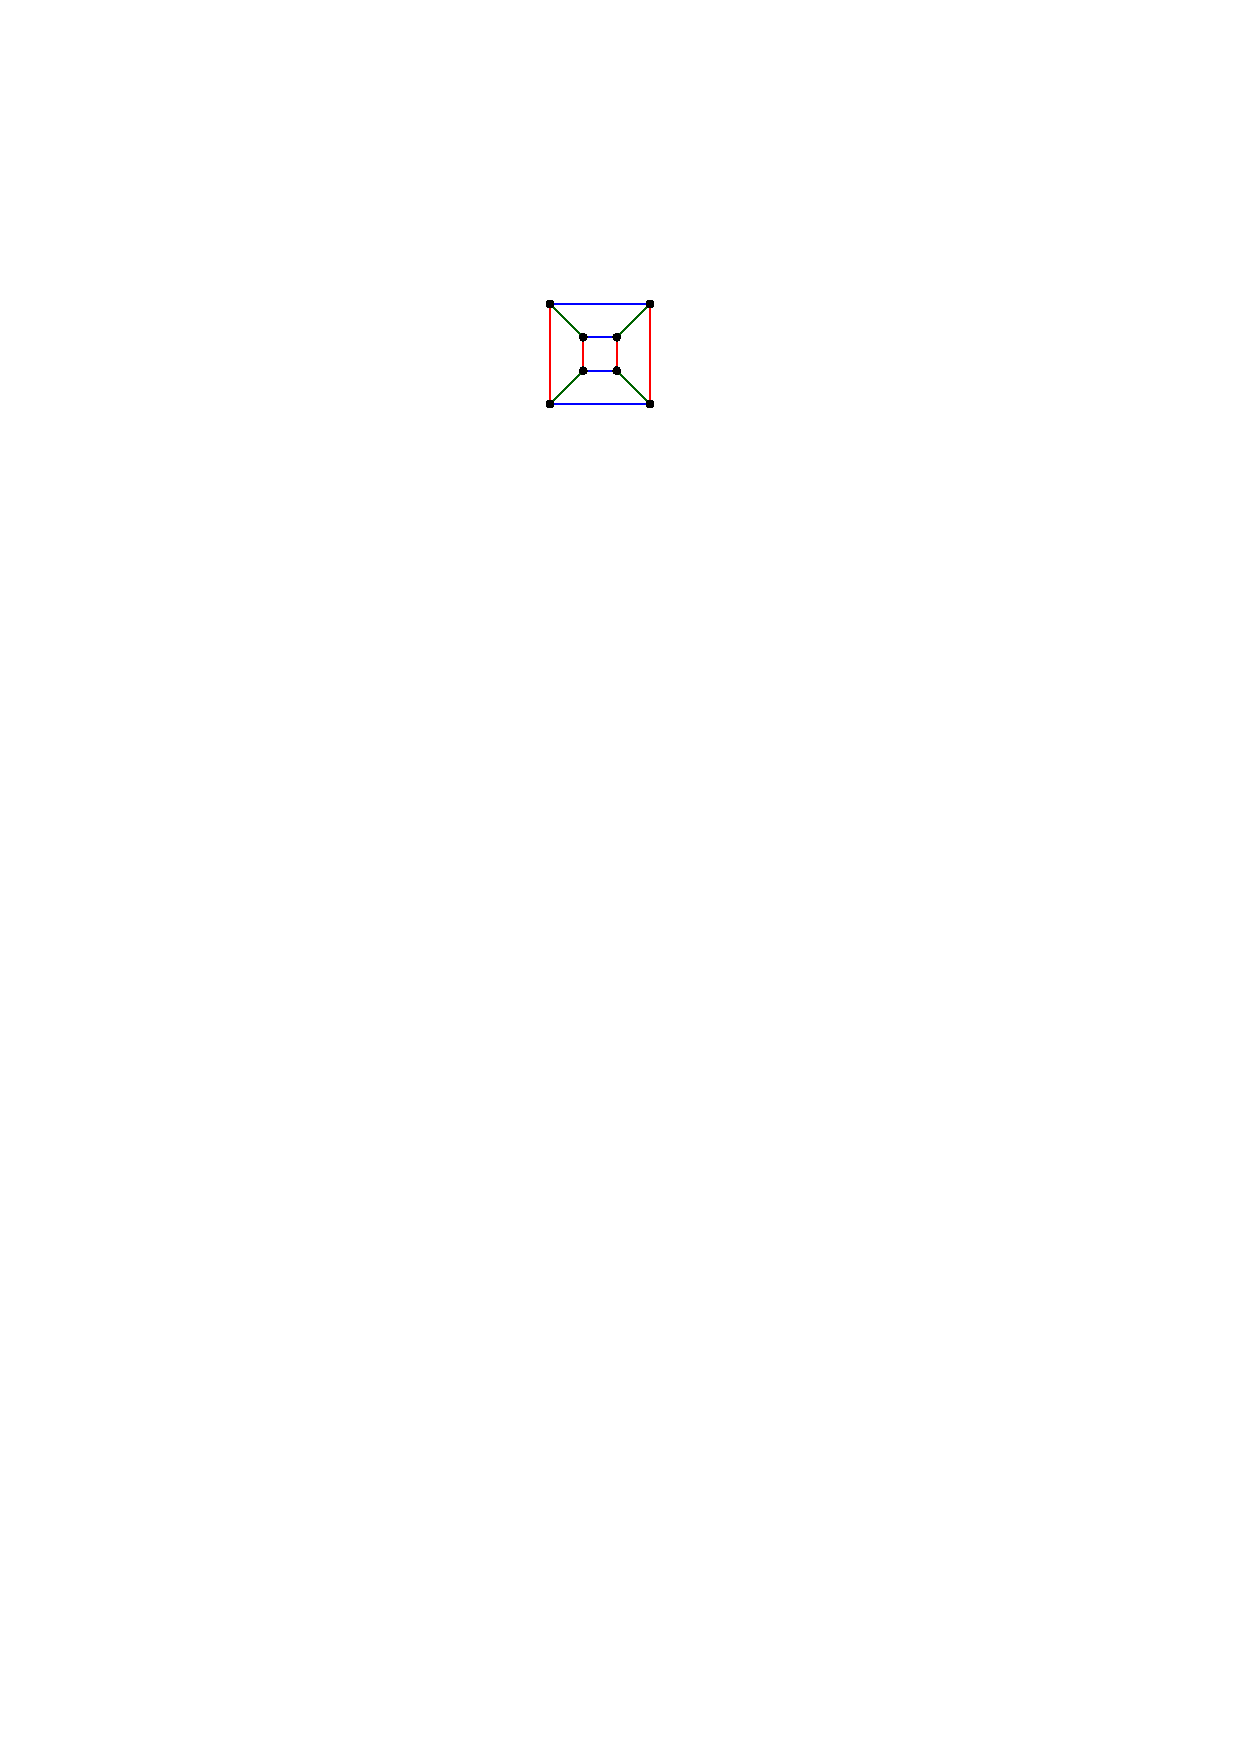
\includegraphics[width=0.2\textwidth]{../Resources/Figs/cubical_edg_colr.pdf}
    \caption{Edge coloring of cubical graph}
    \label{fig:cubical_edge_coloring}
\end{figure}

\subsection{Computed vertex and edge chromatic numbers}

%\todo[inline]{JH: Přidány odkazy na použité funkce a poslední věta zmiňující chromatic index}
%\begin{highlight}
The vertex and edge chromatic numbers can be computed in little time using \textit{SageMath} functions \cite{sagemath-chromatic-number} \cite{sagemath-chromatic-index}. The following two tables provide overview of vertex chromatic numbers $\chi(G)$  and edge chromatic numbers $\chi'(G)$ for Platonic and Archimedean solids. Note that the edge chromatic number $\chi'(G)$ is also called the \textit{chromatic index}.
%\end{highlight}

\begin{table}[H]
    \centering
    \caption{Vertex and edge chromatic numbers of Platonic graphs}
    \vspace{5pt}
    \label{tab:platonic-chrom-nums}
    \begin{tabular}{|l|c|c|}
    \hline
    Platonic & $\chi(G)$ & $\chi'(G)$ \\
    \hline\hline
    cube & 2 & 3 \\
    \hline
    dodecahedron & 3 & 3 \\
    \hline
    icosahedron & 4 & 5 \\
    \hline
    octahedron & 3 & 4 \\
    \hline
    tetrahedron & 4 & 3 \\
    \hline
    \end{tabular}
\end{table}

\begin{table}[H]
    \centering
    \caption{Vertex and edge chromatic numbers of Archimedean graphs}
    \vspace{5pt}
    \label{tab:archimedean-chrom-nums}
    \begin{tabular}{|l|c|c|}
    \hline
    Archimedean & $\chi(G)$ & $\chi'(G)$ \\
    \hline\hline
    cuboctahedron & 3 & 4 \\
    \hline
    icosidodecahedron & 3 & 4 \\
    \hline
    rhombicosidodecahedron & 3 & 4 \\
    \hline
    rhombicuboctahedron & 3 & 4 \\
    \hline
    snub cube & 3 & 5 \\
    \hline
    snub dodecahedron & 4 & 5 \\
    \hline
    truncated cube & 3 & 3 \\
    \hline
    truncated cuboctahedron & 2 & 3 \\
    \hline
    truncated dodecahedron & 3 & 3 \\
    \hline
    truncated icosahedron & 3 & 3 \\
    \hline
    truncated icosidodecahedron & 2 & 3 \\
    \hline
    truncated octahedron & 2 & 3 \\
    \hline
    truncated tetrahedron & 3 & 3 \\
    \hline
    \end{tabular}
\end{table}

Note, that from the tables above, we see that indeed all the above graphs have $\chi(G)$ at most 4. This is due to the famous \textit{Four Color Theorem} \cite{appelhaken76} for planar graphs.

\begin{highlight}

As a consequence of \textit{Vizing's theorem} \cite{misra92}, for every graph $G$ with maximum degree $\Delta(G)$, we have $\Delta(G) \leq \chi'(G) \leq \Delta(G) + 1$. This implies two classes of graphs. Class one are graphs s.t. $\chi'(G) = \Delta(G)$. Class two are then graphs s.t. $\chi'(G) = \Delta(G) + 1$. What class are graphs of Platonic and Archimedean solids?

Let us compare the degrees at each vertex of the solids as shown in tables \ref{tab:platonic-basic-props} and \ref{tab:archimedean-basic-props} with their calculated chromatic indices in the tables above. It turns out, that all the solids are of Vizing class one. Note that this is not the case for all planar graphs. In fact, there exist planar graphs with $\Delta(G)$ up to 5 such that they are class two.

\end{highlight}

\subsection{Total coloring}

\begin{definition}
    A \textit{total coloring} of graph $G=(V,E)$ is a coloring $c: V \cup E \rightarrow \mathbb{N}$ from family of colorings sharing both coloring rules \ref{eqn:vtx_rule} and \ref{eqn:edge_rule} and the following additional rule: 
    \begin{equation}\label{eqn:tot_rule}
    \forall v \in V,  \forall e \in E, \text{ if } \{v\} \cap e \neq \emptyset \text{ then } c(v) \neq c(e) \tag{$R_T$}
    \end{equation}
    We will call this family $F_T$.
\end{definition}

\begin{figure}[H]
    \centering
    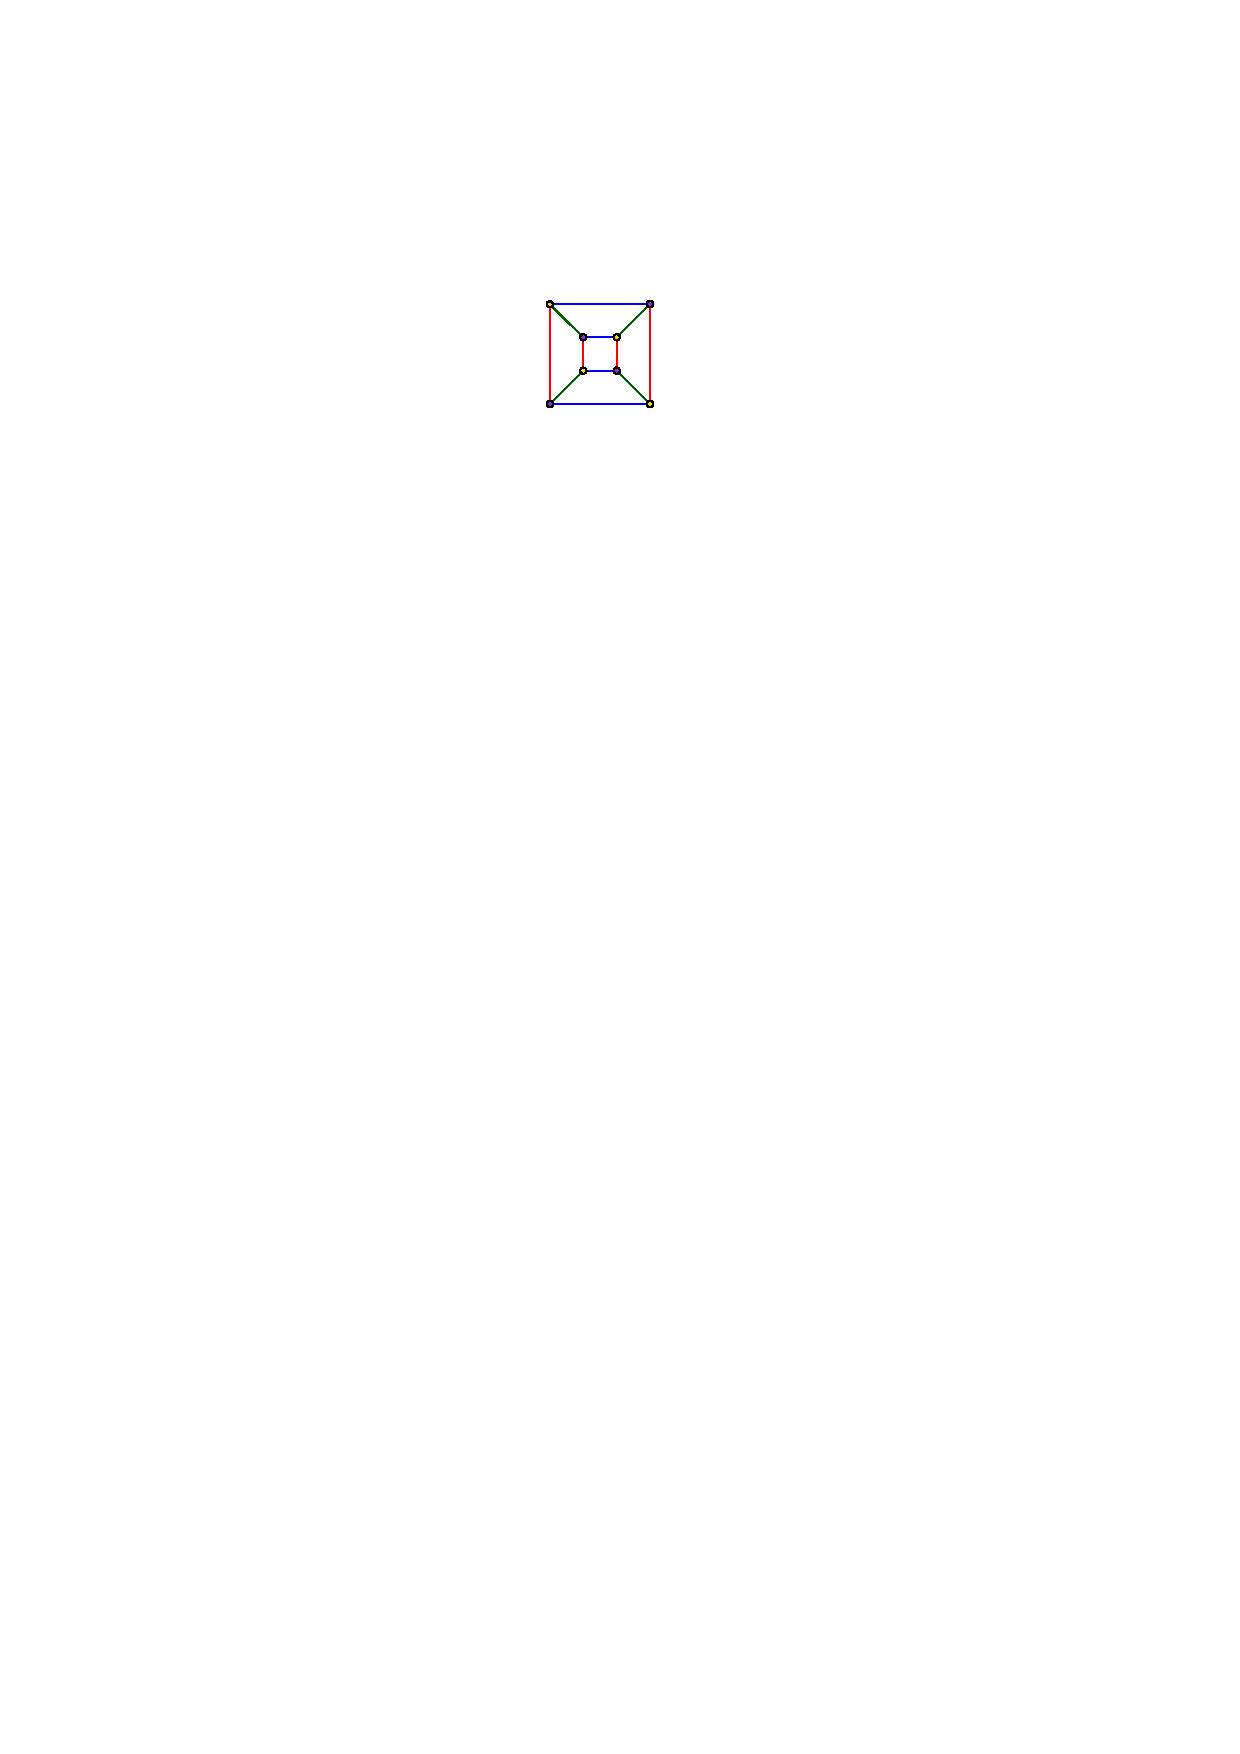
\includegraphics[width=0.2\textwidth]{../Resources/Figs/cubical_tot_colr.pdf}
    \caption{Total coloring of cubical graph using five colors}
    \label{fig:cubical_tot_coloring}
\end{figure}

\begin{figure}[H]
    \centering
    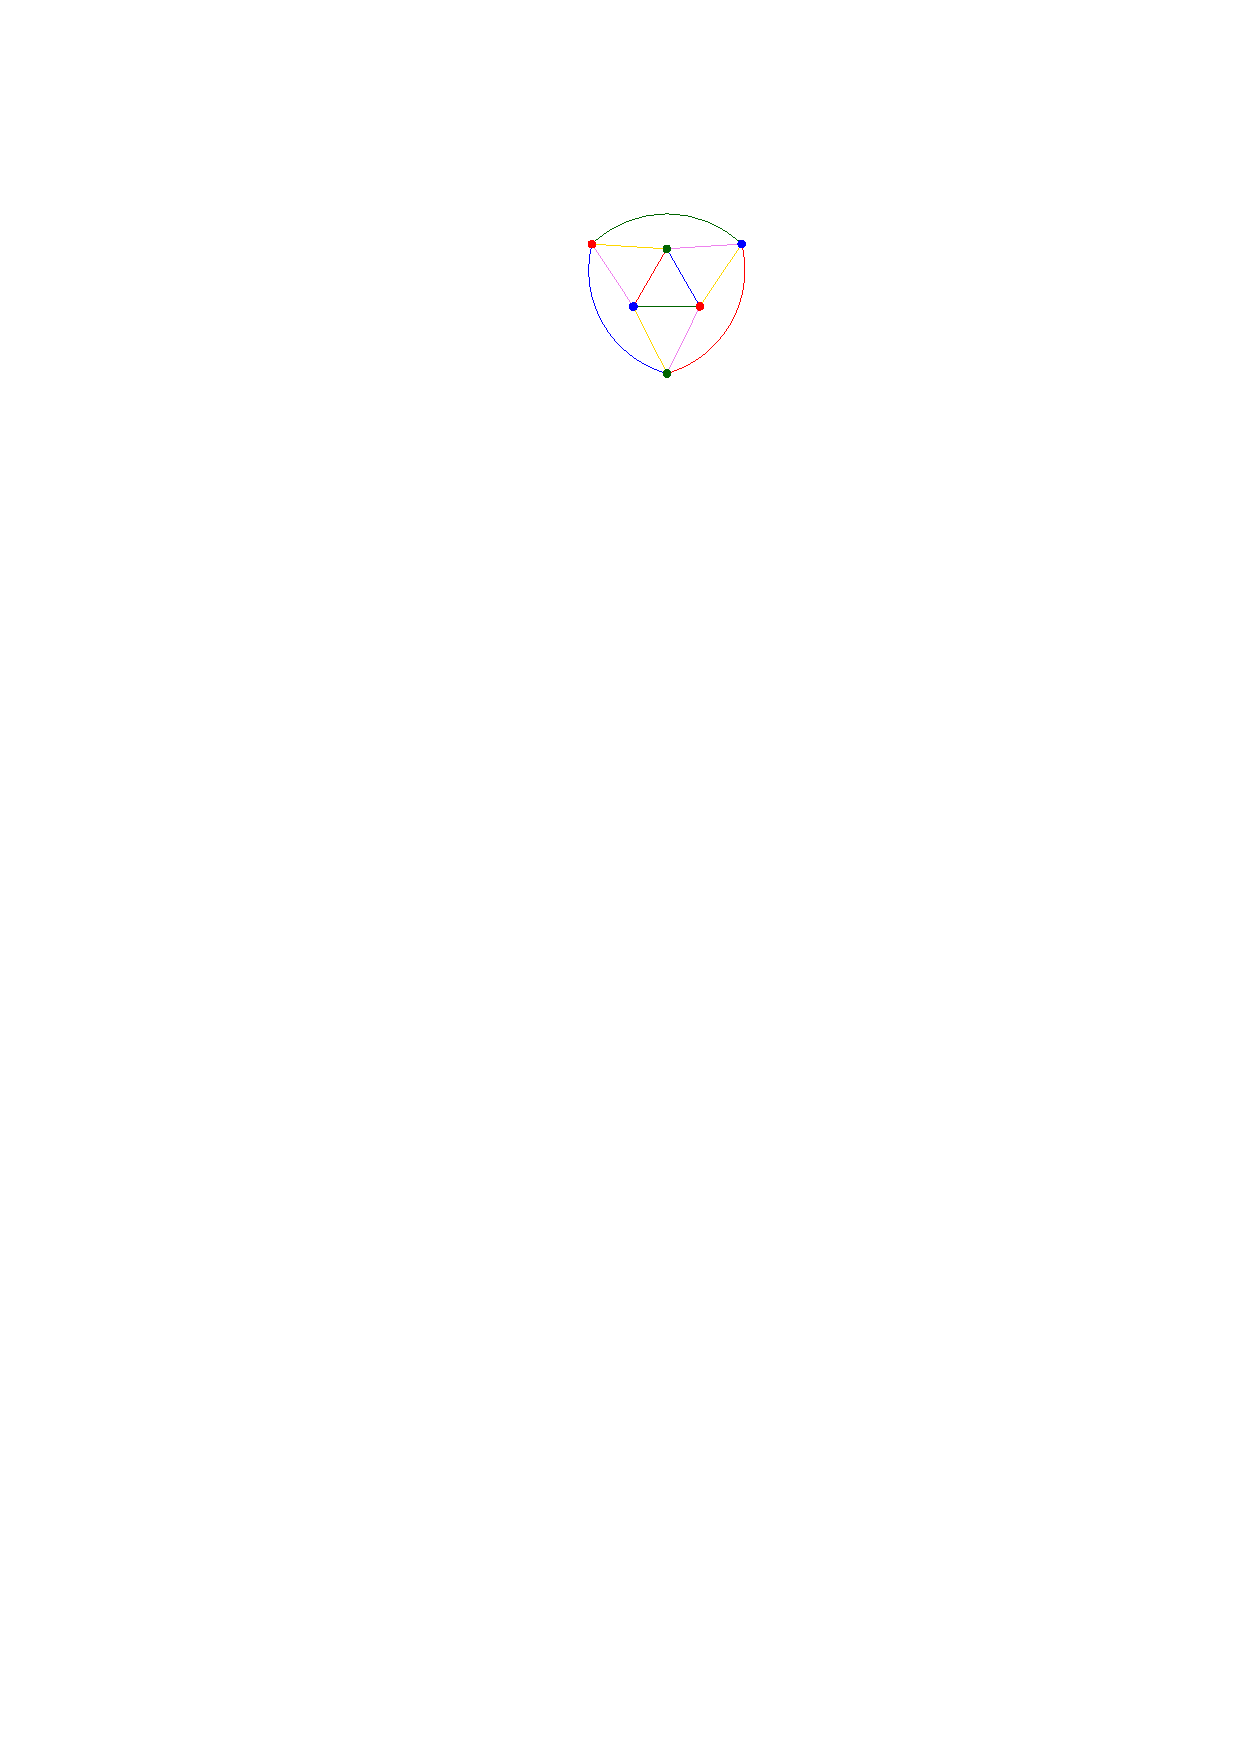
\includegraphics[width=0.2\textwidth]{../Resources/Figs/octahedral_tot_colr.pdf}
    \caption{Total coloring of octahedral graph using five colors}
    \label{fig:octahedral_tot_coloring}
\end{figure}

\todo[inline]{TODO: Rainbow coloring a magic labeling -  těmto konceptům se věnovat nejspíš nebudeme, ale bylo by dobré je zmínit někde v úvodu jako barvení, kde jsou ještě další podmínky, resp. kdy hraje roli, jakou hodnotu mají použité barvy.}

\todo{JF: Námět: popsat jak lze od složitějších přecházet ke klasickému vrcholovému - přes linegraf, graf incidencí, duál  apod., kdyžtak vysvětlím zítra. Možná se ukáže, že to pro sage bude snazší redukovat na vrcholové obarvení, možná i se zkoumáním symetrií.}




\subsection{Some calculated chromatic polynomials}
\todo[inline]{NOTE: The following tables will most likely not be in the final thesis. Since there is not much interesting that one can see from them.}
\begin{table}[H]
\centering
\begin{tabular}{|l|p{0.5\linewidth}|}
\hline
Platonic & chromatic polynomial \\
\hline\hline
cube & $x^{8} - 12x^{7} + 66x^{6} - 214x^{5} + 441x^{4} - 572x^{3} + 423x^{2} - 133x$ \\
\hline
dodecahedron & $x^{20} - 30x^{19} + 435x^{18} - 4060x^{17} + 27393x^{16} - 142194x^{15} + 589875x^{14} - 2004600x^{13} + 5673571x^{12} - 13518806x^{11} + 27292965x^{10} - 46805540x^{9} + 68090965x^{8} - 83530946x^{7} + 85371335x^{6} - 71159652x^{5} + 46655060x^{4} - 22594964x^{3} + 7171160x^{2} - 1111968x$ \\
\hline
icosahedron & $x^{12} - 30x^{11} + 415x^{10} - 3500x^{9} + 20023x^{8} - 81622x^{7} + 241605x^{6} - 517360x^{5} + 780286x^{4} - 782108x^{3} + 463310x^{2} - 121020x$ \\
\hline
octahedron & $x^{6} - 12x^{5} + 58x^{4} - 137x^{3} + 154x^{2} - 64x$ \\
\hline
tetrahedron & $x^{4} - 6x^{3} + 11x^{2} - 6x$ \\
\hline
\end{tabular}
\end{table}
\begin{table}[H]
\centering
\begin{tabular}{|l|p{0.5\linewidth}|}
\hline
Archimedean & chromatic polynomial \\
\hline\hline
cuboctahedron & $x^{12} - 24x^{11} + 268x^{10} - 1842x^{9} + 8680x^{8} - 29516x^{7} + 74019x^{6} - 136826x^{5} + 182024x^{4} - 164656x^{3} + 90016x^{2} - 22144x$ \\
\hline
icosidodecahedron & $None$ \\
\hline
rhombicosidodecahedron & $None$ \\
\hline
rhombicuboctahedron & $None$ \\
\hline
snub cube & $None$ \\
\hline
snub dodecahedron & $None$ \\
\hline
truncated cube & $x^{24} - 36x^{23} + 622x^{22} - 6868x^{21} + 54445x^{20} - 330016x^{19} + 1590616x^{18} - 6258826x^{17} + 20483524x^{16} - 56517092x^{15} + 132781696x^{14} - 267560902x^{13} + 464751928x^{12} - 698041384x^{11} + 907685011x^{10} - 1021028578x^{9} + 990348490x^{8} - 822946048x^{7} + 579284763x^{6} - 338935770x^{5} + 159596344x^{4} - 57088336x^{3} + 13839584x^{2} - 1703168x$ \\
\hline
truncated cuboctahedron & $None$ \\
\hline
truncated dodecahedron & $None$ \\
\hline
truncated icosahedron & $None$ \\
\hline
truncated icosidodecahedron & $None$ \\
\hline
truncated octahedron & $x^{24} - 36x^{23} + 630x^{22} - 7134x^{21} + 58707x^{20} - 373816x^{19} + 1914823x^{18} - 8098890x^{17} + 28806937x^{16} - 87308340x^{15} + 227623087x^{14} - 513887650x^{13} + 1008990864x^{12} - 1726780052x^{11} + 2576178723x^{10} - 3343211267x^{9} + 3755216148x^{8} - 3618864524x^{7} + 2949553512x^{6} - 1987203924x^{5} + 1066396109x^{4} - 427989031x^{3} + 114056146x^{2} - 15071023x$ \\
\hline
truncated tetrahedron & $x^{12} - 18x^{11} + 149x^{10} - 752x^{9} + 2586x^{8} - 6408x^{7} + 11774x^{6} - 16189x^{5} + 16468x^{4} - 11869x^{3} + 5442x^{2} - 1184x$ \\
\hline
\end{tabular}
\end{table}
